%%
%% This is file `sample-manuscript.tex',
%% generated with the docstrip utility.
%%
%% The original source files were:
%%
%% samples.dtx  (with options: `manuscript')
%% 
%% IMPORTANT NOTICE:
%% 
%% For the copyright see the source file.
%% 
%% Any modified versions of this file must be renamed
%% with new filenames distinct from sample-manuscript.tex.
%% 
%% For distribution of the original source see the terms
%% for copying and modification in the file samples.dtx.
%% 
%% This generated file may be distributed as long as the
%% original source files, as listed above, are part of the
%% same distribution. (The sources need not necessarily be
%% in the same archive or directory.)
%%
%% Commands for TeXCount
%TC:macro \cite [option:text,text]
%TC:macro \citep [option:text,text]
%TC:macro \citet [option:text,text]
%TC:envir table 0 1
%TC:envir table* 0 1
%TC:envir tabular [ignore] word
%TC:envir displaymath 0 word
%TC:envir math 0 word
%TC:envir comment 0 0
%%
%%
%% The first command in your LaTeX source must be the \documentclass command.
%%\documentclass[manuscript,screen,review,nonacm]{acmart}
\documentclass[sigplan,screen]{acmart}
\usepackage{hyperref,xurl}
\usepackage{natbib}
\usepackage{colortbl}
\usepackage{graphicx}
\usepackage{subcaption}
%%
%% \BibTeX command to typeset BibTeX logo in the docs
\AtBeginDocument{%
  \providecommand\BibTeX{{%
    \normalfont B\kern-0.5em{\scshape i\kern-0.25em b}\kern-0.8em\TeX}}}

%% Rights management information.  This information is sent to you
%% when you complete the rights form.  These commands have SAMPLE
%% values in them; it is your responsibility as an author to replace
%% the commands and values with those provided to you when you
%% complete the rights form.
\setcopyright{acmcopyright}
\copyrightyear{2023}
\acmYear{2023}
\acmDOI{XXXXXXX.XXXXXXX}

%% These commands are for a PROCEEDINGS abstract or paper.
\acmConference[CS 235]{Data Mining Techniques}{Fall 2023}{University of California, Riverside}
% \acmPrice{15.00}
% \acmISBN{978-1-4503-XXXX-X/18/06}


%%
%% Submission ID.
%% Use this when submitting an article to a sponsored event. You'll
%% receive a unique submission ID from the organizers
%% of the event, and this ID should be used as the parameter to this command.
%%\acmSubmissionID{123-A56-BU3}

%%
%% For managing citations, it is recommended to use bibliography
%% files in BibTeX format.
%%
%% You can then either use BibTeX with the ACM-Reference-Format style,
%% or BibLaTeX with the acmnumeric or acmauthoryear sytles, that include
%% support for advanced citation of software artefact from the
%% biblatex-software package, also separately available on CTAN.
%%
%% Look at the sample-*-biblatex.tex files for templates showcasing
%% the biblatex styles.
%%

%%
%% The majority of ACM publications use numbered citations and
%% references.  The command \citestyle{authoryear} switches to the
%% "author year" style.
%%
%% If you are preparing content for an event
%% sponsored by ACM SIGGRAPH, you must use the "author year" style of
%% citations and references.
%% Uncommenting
%% the next command will enable that style.
%%\citestyle{acmauthoryear}

%%
%% end of the preamble, start of the body of the document source.
\begin{document}

%%
%% The "title" command has an optional parameter,
%% allowing the author to define a "short title" to be used in page headers.
\title{CS235 Fall'23 Project Final Report: Use Deep Learning to Predict Car Sales Price}

\author{Liam Hsieh}
\affiliation{%
  \institution{University of California, Riverside}
  \streetaddress{900 University Ave}
  \city{Data Science, MSOL}\\
  \state{862395843}
  \country{}
}
\email{lhsie013@ucr.edu}

\renewcommand{\shortauthors}{Liam Y. Hsieh}

%%
%% The abstract is a short summary of the work to be presented in the
%% article.
\begin{abstract}
This project leverages Artificial Neural Networks (ANNs) to predict car sales prices, comparing their performance against linear regression. The selected ANN model, with three hidden layers (5-10-5) and a linear activation function, outperforms linear regression in Mean Absolute Error. The project follows a systematic flow, encompassing data preprocessing, model exploration, and final evaluation. Visualizations support the model selection, contributing valuable insights to the automotive industry
\end{abstract}

%%
%% Keywords. The author(s) should pick words that accurately describe
%% the work being presented. Separate the keywords with commas.
\keywords{Car sales price prediction, Neural Networks, Mean Absolute Error (MAE)}


%%
%% This command processes the author and affiliation and title
%% information and builds the first part of the formatted document.
\maketitle

\section{Introduction}

\urldef{\dataurl}\url{https://www.kaggle.com/datasets/yashpaloswal/ann-car-sales-price-prediction}

The proposed project aims to leverage Deep Learning to predict car sales prices based on a dataset obtained from Kaggle \footnote{\dataurl}. The dataset consists of 500 records with 9 columns, encompassing customer details such as name, email, country, gender, age, annual salary, credit card debt, net worth, and car purchase amount. The objective is to explore the potential of ANN models in predicting car sales prices compared to a baseline model using linear regression. Linear regression will serve as the benchmark model, and various ANN structures will be evaluated to identify the most suitable and accurate predictive model. By harnessing the capabilities of ANN, we aim to enhance the accuracy and precision of car sales price predictions, providing valuable insights for the automotive industry and aiding customers in making informed purchasing decisions.




\section{Related Work}
The prediction of car prices using machine learning has attracted considerable attention. Cars, being both ubiquitous and essential commodities in the modern world, possess well-known features familiar to most people. The pricing of cars shows a clear correlation with several features, contributing to the popularity of applying machine learning for predicting car prices. One prevalent application involves forecasting the retail or invoice price of cars based on features and dealer information, especially in the context of used cars \citep{asghar2021used, narayana2022second}.

During the COVID-19 pandemic, with a shortage of vehicles in the market, the prices of used cars experienced a significant boost. This surge has led many individuals to seek scientific references to aid in decision-making. Consequently, there is a growing demand for machine learning-based methods to address this need.

Given the strong linear relationship between features and price, linear regression has proven to be effective in predicting car prices \citep{bukvic2022price, sumeyra2023using}.

\section{Proposed Approach} 

The proposed approach involves initially splitting the dataset into a training set (80\%) and a testing set (20\%). The core of the project revolves around leveraging Artificial Neural Networks (ANNs) to predict car sales prices. The ANN architecture comprises an input layer representing selected features, multiple hidden layers activated using linear functions, and an output layer for regression, employing the mean absolute error loss. The Keras library, built on TensorFlow, will be utilized to implement the ANN model. Specifically, the output layer will employ a linear activation function to predict numeric car purchase amounts. Different activation functions, e.g., {\it relu},{\it sigmoid}, and {\it linear}, number of hidden layers, and optimizers, e.g., {\it adam},{\it sgd}, and {\it nadam}, including will be explored and compared to determine the most effective model configuration. The ANN model will be compiled using a defined optimizer and loss function, and subsequently trained on the training set. Evaluation of the ANN's performance will be conducted using the testing set. After a screening experiment for different optimizers, number of neurons, and activate functions, we further applied cross validation to determine the potential of adding additional hidden layers from just two to five and to select the most accurate and efficient model for car sales price prediction.

The model we eventually used for the prediction is described as follows:

\begin{itemize}
  \item three hidden layers.
  \item number of neurons for each hidden layers are 5, 10, and 5, sequentially.
  \item the activate function is linear for each layer.
  \item optimizer is adam.
  \item number of epochs for model training is 80 and batch size is 64. 
\end{itemize}

Fig. \ref{fig:training} is the lost plot for the proposed ANN model.

\begin{figure}[h]
  \centering
  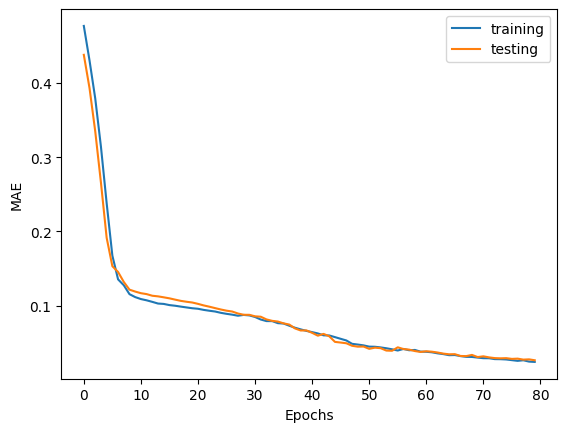
\includegraphics[width=0.8\linewidth]{training.png}
  \caption{ANN training loss vs testing loss plot}
  \label{fig:training}
\end{figure}


\begin{figure}[h]
  \centering
  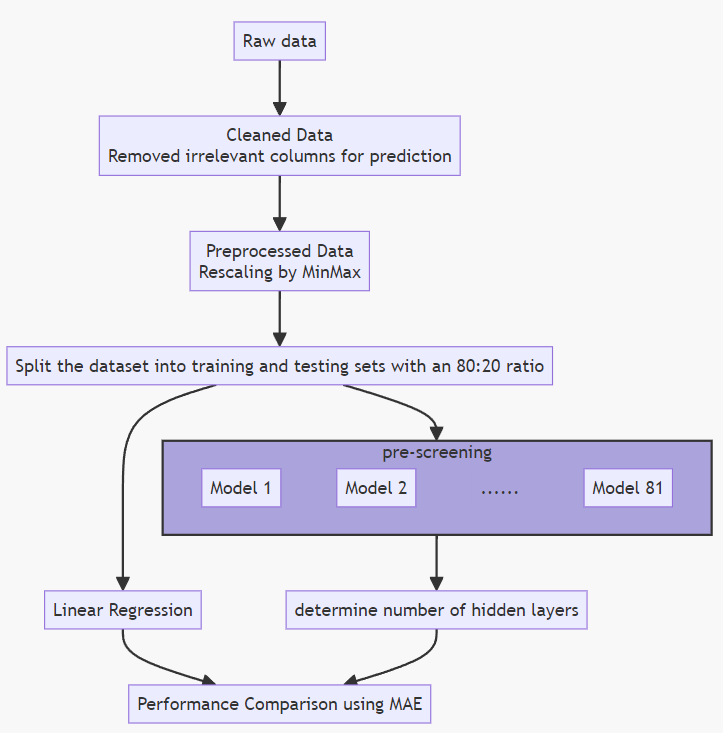
\includegraphics[width=0.8\linewidth]{flowchart.png}
  \caption{Project Overview.}
  \label{fig:flowchart}
\end{figure}

The high-level flow for proposed approach is shown as Fig. \ref{fig:flowchart}. The presented flowchart outlines the sequential steps in a data-driven predictive modeling process. It begins with raw data, progresses through data cleaning and preprocessing, including MinMax normalization. The dataset is then split into training and testing sets with an 80:20 ratio. Two main branches of modeling are pursued: one involves Linear Regression as baseline, and the other conducts a pre-screening with 81 distinct Artificial Neural Network (ANN) models to narrow down the exploration then determine the number of hidden layers later. The final step involves a comprehensive evaluation of model performance using Mean Absolute Error, providing a comparative analysis between Linear Regression and various ANN models.

The results of pre-screening have been illustrated by Fig. \ref{fig:prescreen_output} it helps narrow down those low performance model configuration rapidly before we moved to determine the number of hidden layers.

\begin{figure}
  \centering
  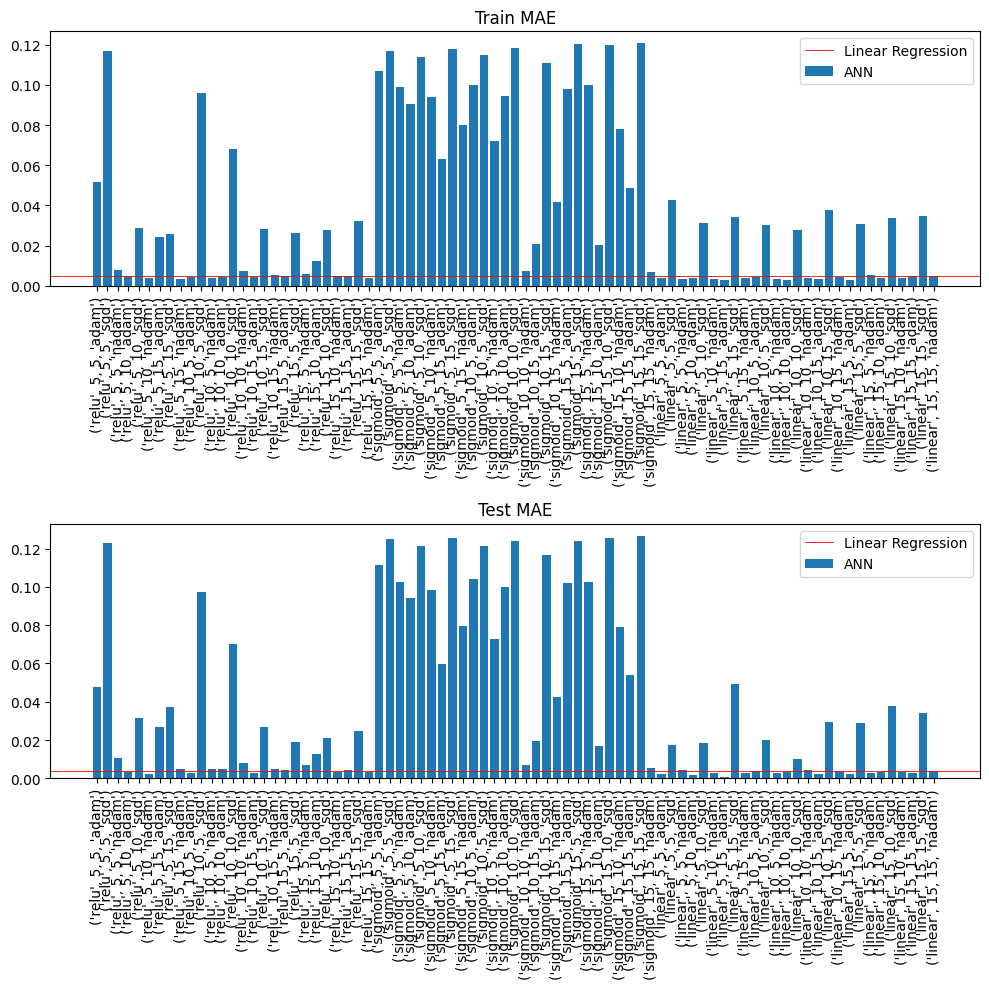
\includegraphics[width=0.8\linewidth]{prescreening_output.png}
  \caption{Output Overview}
  \label{fig:prescreen_output}
\end{figure}


Moreover, Fig. \ref{fig:boxplot} and Fig. \ref{fig:layers} support our decision of selecting the 3-layers-linear as our prediction model because it not only has the lowest average MAE but also has smallest standard deviation of MAE.

\begin{figure}
    \begin{subfigure}{0.5\textwidth}
        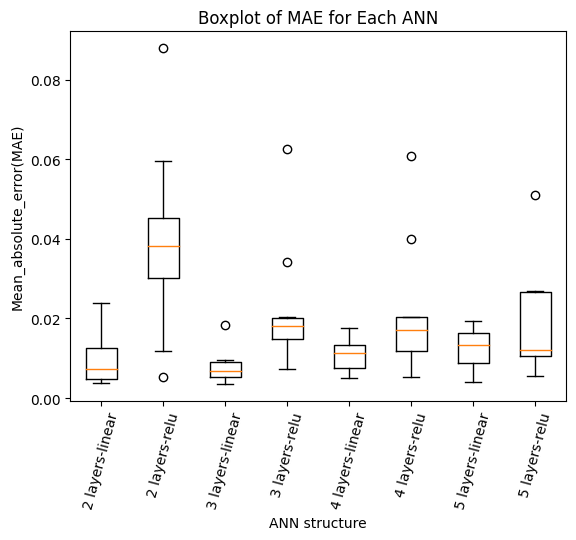
\includegraphics[width=\linewidth]{boxplot.png}
        \caption{Boxplot of different ANN models}
        \label{fig:boxplot}
    \end{subfigure}
    \begin{subfigure}{0.5\textwidth}
        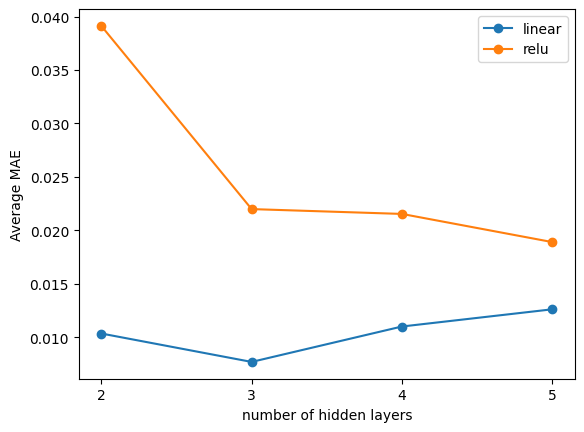
\includegraphics[width=\linewidth]{layers.png}
        \caption{Mean MAE of ANN Models with Varying Number of Hidden Layers}
        \label{fig:layers}
    \end{subfigure}
    \caption{Comparison of ANN models.}
    \label{fig:comparison}
\end{figure}



\section{DISCUSSION and CONCLUSIOINS}
This paper proposed a multi-layers artificial neural network model to predict car sales price and implement from scratch using Keras. Comparing to the performance of linear regression, the most common prediction method in this kind of problem due to strong linearity, the proposed model can outperform linear regression by mean absolute error.
\bibliographystyle{ACM-Reference-Format}
\bibliography{reference}
\end{document}
\endinput
%%
%% End of file `sample-manuscript.tex'.
